\section{Propriétés réfléctives des élements à capturer}
Durant ses activités, le système observera principalement les élements suivants:
\begin{enumerate}
    \item Les hydrocarbures
    \item Le béton
    \item Le goudron
\end{enumerate}
On m'informant sur les méthodes de détection déjà existante des hydrocarbures, j'ai constaté que l'intégralité d'entre eux fonctionnent
par ultraviolet (mesure de fluoresence) et par infrarouge. Je vais donc m'informer sur la réaction des éléments susmentionné suivant l'exposition à différentes longueurs d'ondes.
\subsection{Hydrocarbures}
Les principaux hydrocarbures traités par les pompiers durant leurs interventions sont les suivants:
\begin{enumerate}
    \item L'huile de moteur.
    \item L'huile hydraulique (tracteur).
    \item L'essence \cite{TotalEnergies}.
    \item Le diesel \cite{TotalEnergies}.
\end{enumerate}
Les éléments principaux qui les composent sont les suivants:
\begin{itemize}
    \item Les alcènes
    \item Les alcanes
    \item Les hydrocarbures aromatiques
\end{itemize}
Divers travaux \cite{Hydrocarbures} traitent des spectres IR des hydrocarbures, mettant en relation la transmittance des éléments en fonction de la longueur d'onde.
Tirés desdits travaux, les graphiques suivants délivres des informations utiles sur la problèmatique du projet.

\begin{figure}[H]
    \centering
    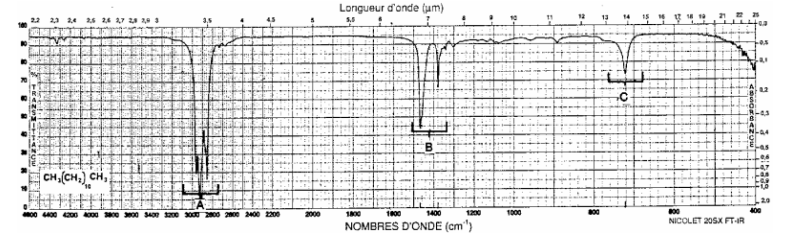
\includegraphics[height=7cm,angle=90]{assets/figures/alcanes1.png}
    \caption{Alcanes - spectre IR du dodécane \cite{Hydrocarbures}}
\end{figure}

\begin{figure}[H]
    \centering
    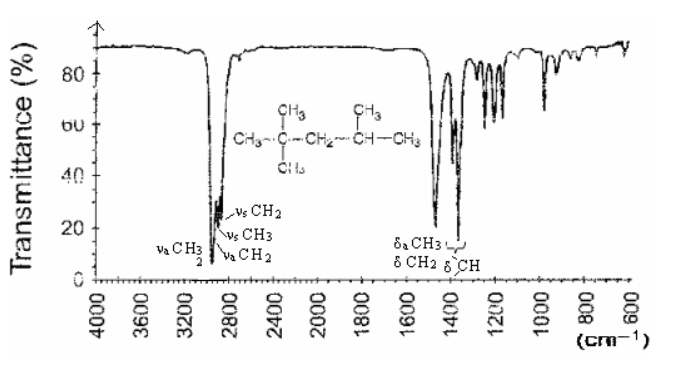
\includegraphics[height=6cm,angle=90]{assets/figures/alcanes2.png}
    \caption{Alcanes - spectre IR du triméthyl-pentane \cite{Hydrocarbures}}
\end{figure}

\begin{figure}[H]
    \centering
    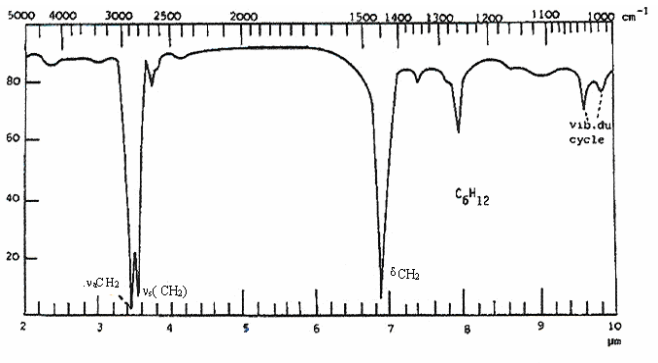
\includegraphics[height=5cm,angle=90]{assets/figures/alcanes3.png}
    \caption{Alcanes - spectre IR du cycloalcanes \cite{Hydrocarbures}}
\end{figure}

\begin{figure}[H]
    \centering
    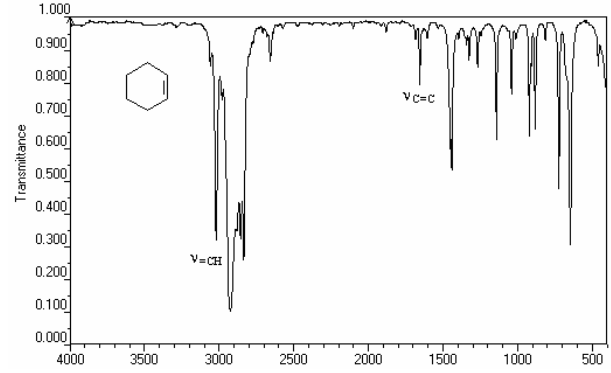
\includegraphics[height=5cm,angle=90]{assets/figures/alcenes1.png}
    \caption{Alcènes - spectre IR du cyclohexène \cite{Hydrocarbures}}
\end{figure}

\begin{figure}[H]
    \centering
    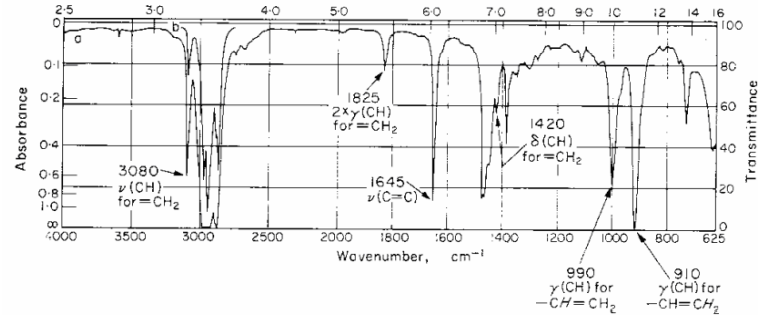
\includegraphics[height=5cm,angle=90]{assets/figures/alcenes2.png}
    \caption{Alcanes - spectre IR du  1-octène à l’état liquide\cite{Hydrocarbures}}
\end{figure}

\begin{figure}[H]
    \centering
    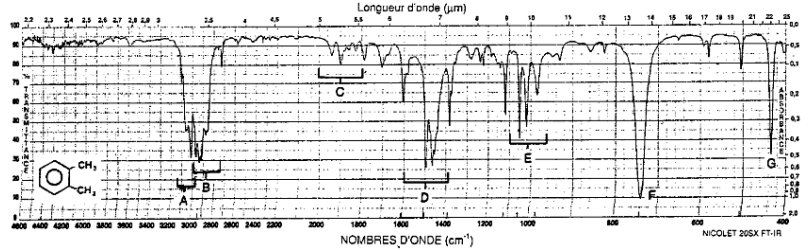
\includegraphics[height=5cm,angle=90]{assets/figures/aromatique.png}
    \caption{Aromatique - spectre IR du o-xylène \cite{Hydrocarbures}}
\end{figure}

\newpage
La transmittance indiquée sur l'axe de l'ordonnée représente l'inverse de l'absorbption, c'est à dire que si la transmittance est faible, la lumière
est "très" absorbée par l'hydrocarbure et inversement, si la transmittance est élevée, la lumière est "peu" absorbée par l'hydrocarbure, la laissant ainsi traverser.
Nous observons un point commun pour les trois types d'hydrocarbures, il s'agit des pics d'absorbptions aux alentours de \underline{3000 \si{\per\centi\metre}}, ce qui correspond à \underline{3300 \si{\nano\metre}}.

Pour cette longueur d'onde spécifique, la transmittance globale se trouve entre \underline{5 et 30\%}.

\subsection{Béton}

\subsection{Goudron}
On retrouve des hydrocarbures dans la composition du goudron, ceux-ci étant similaires aux hydrocarbures à détecter, le spectre IR pourrait nous indiquer des problèmes de détection pour la classification ...

\subsection{Bitume}
Des informations sont disponibles certains travaux en ligne \cite{Bitume}. Le graphe suivant met en évidence les pics d'absorbption du bitume.

\begin{figure}[H]
    \centering
    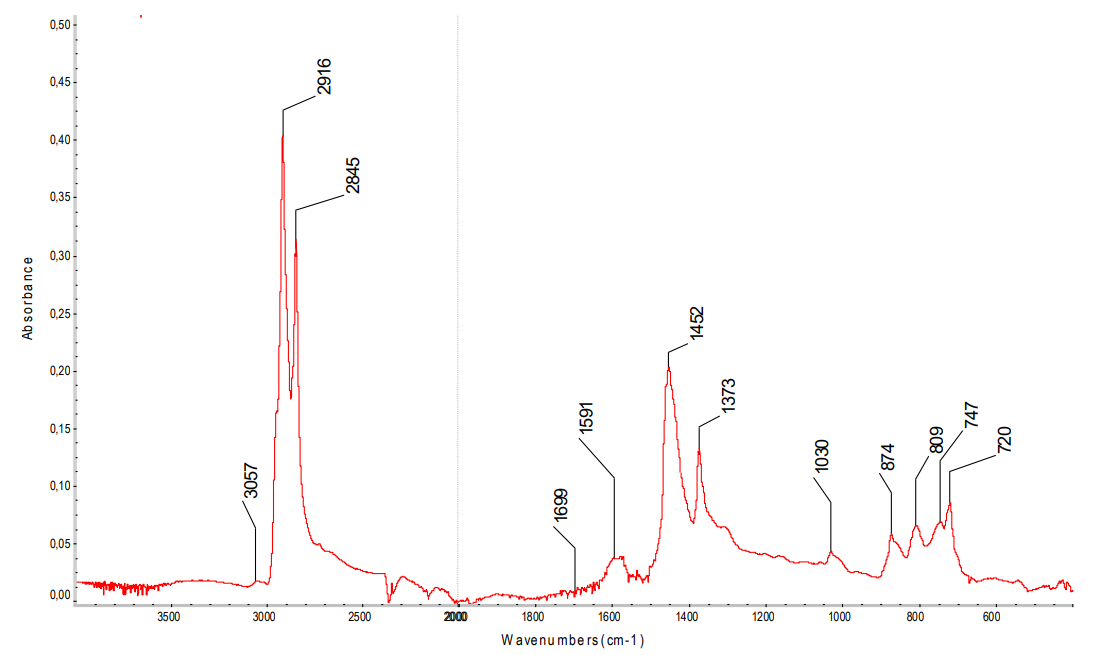
\includegraphics[width=13cm]{assets/figures/bitumeIR.png}
    \caption{Bitume - Spectre IR \cite{Bitume}}
\end{figure}

\subsection{Analyse}
On observe que les diverses élements qui seront vus par la caméra ont une variation du taux d'absorptions face aux longueurs d'onde avoisinant les
3300 \si{\nano\metre}, mais à différents ordres de grandeurs. Là ou les hydrocarbures absorbent jusqu'à 95\% des ondes, les routes en absorbent "seulement" jusqu'à 45\%.
En se basant sur ceci, il devrait être possible de faire une différenciation par l'intermédiaire d'un capteur adapté.


Selon les normes \Gls{iso} 20473:2007 \cite{ISO}, cette longueur d'onde se trouve parmi les \Gls{mir}.
\begin{figure}[H]
    \centering
    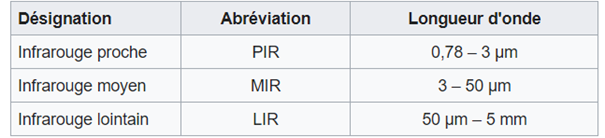
\includegraphics[width=13cm]{assets/figures/gamme_infra.png}
    \caption{Classification des \Gls{ir} selon les normes \Gls{iso} 20473:2007 \cite{ISO}}
\end{figure}

Après quelques recherches à propos d'un éclairage et surtout d'un capteur adapté à cette gamme de longueur d'onde, je me suis vite aperçu
que les disponibilités et les délais d'arrivée de ce genre de composants ne correspondait pas avec le rythme d'avancée de mon travail,
j'ai donc exploré d'autres options, toujours dans le milieu de l'infrarouge.

Je suis tombé par hasard sur les produits du "Laboratoire des huiles de moteurs" (faisant parti du HTDS), qui apparemment, utilisent
des rayonnements infrarouges proche du visible (aux alentours de 850nm) pour effectuer des analyses. Très peu de documentation est disponible sur le fonctionnement,
mais la disponibilités d'un capteur et d'éclairage pour cette gamme de longueur d'onde permet d'effectuer des tests très rapidement.
Les résultats de ces tests se trouvent au chapitre \ref{test_vision}.

\textbf{Note suites aux essaies: Les tests semblent concluant et ressorte des images tout à fait exploitables pour effectuer une localisation des
    traces d'hydrocarbures.}

\textbf{\underline{La suite du projet se basera sur un éclairage émettant à 850nm.}}